\thispagestyle{empty}
\null
\vfill
\begin{center}
   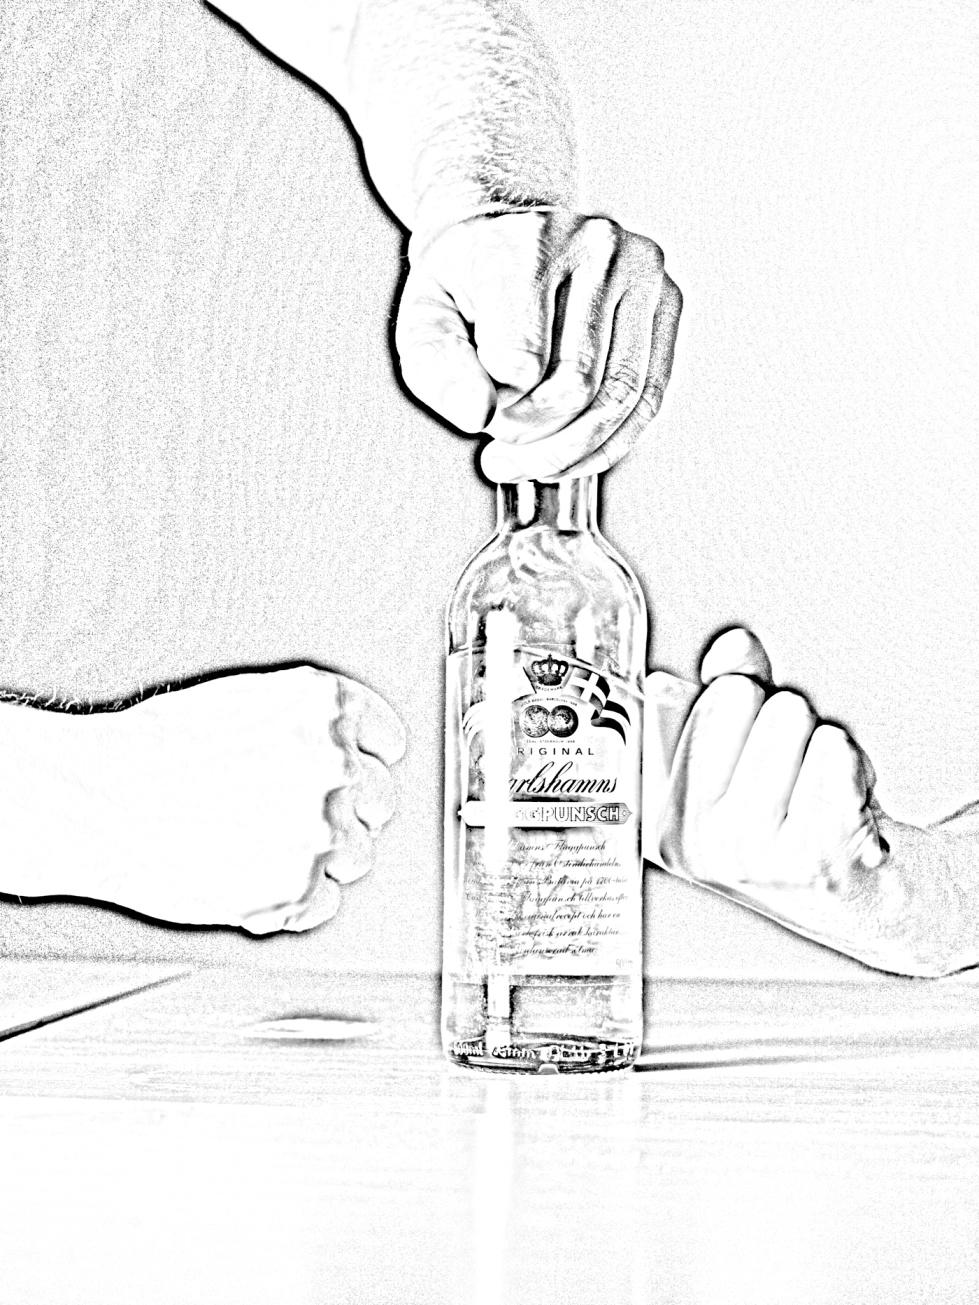
\includegraphics[width=0.9\textwidth]{res/punschvisor.jpg}
   \section{Punschvisor}
\end{center}
\vfill
\newpage

\subsection{Punschen kommer (kall)}
\textit{Mel: Vals ur Glada Änkan}\\
\index[alfa]{Punschen kommer (kall)}
\index[anfa]{Punschen kommer, punschen kommer...}
\begin{parse lines}[\noindent]{#1\\}

Punschen kommer, punschen kommer,
ljuv och sval.
Glasen imma, röster stimma
i vår sal.
Skål för glada minnen!
Skål för varje vår!
Inga sorger finnas mer
när punsch vi får.
\end{parse lines}


\subsection{Punschen kommer (varm)}
\textit{Mel: Vals ur Glada Änkan}\\
\index[alfa]{Punschen kommer (varm)}
\index[anfa]{Punschen kommer, punschen kommer...}
\begin{parse lines}[\noindent]{#1\\}

Punschen kommer, punschen kommer,
god och varm.
Vettet svinner, droppen rinner
ner i tarm.
Skål för glada minnen!
Dem vi snart ej ha,
då ett par glas simmig punsch
vi hunnit ta.
\end{parse lines}

\newpage

\begin{picture}(50,50) \put(155,0){\hbox{
\includegraphics[height=0.15\textheight]{res/kretslopp.png}}} \end{picture}
\vspace*{-0.20\textheight}


\subsection{Kretsloppet}
\textit{Mel: Nu har vi ljus}\\
\index[alfa]{Kretsloppet}
\index[anfa]{Genom vår kropp, ända till snopp...}
\begin{parse lines}[\noindent]{#1\\}

Genom vår kropp, ända till snopp,
punsch håller färgen, hopp, tralalala.
Kolla ditt kiss, ser du, jovisst, ser du, jovisst!
Samma gyllengula ädla vätska,
samma dryck som nyss vår tunga läska
tralalala lalalalala lalalalala lalala.

Tar punschen slut, spar på ditt krut,
skjut inte värden, hopp, tralalala.
Låt punschen gå varv nummer två, varv nummer två:
Två och två ni mot varandra ilar,
snart i munnen punschen åter strilar
tralalala lalalalala lalalalala lalala.
\end{parse lines}


\subsection{Gula droppar}
\textit{Mel: Midnatt råder}\\
\index[alfa]{Gula droppar}
\index[anfa]{Punschen, punschen rinner genom strupen...}
\begin{parse lines}[\noindent]{#1\\}

Punschen, punschen rinner genom strupen,
ner i djupen.
Blandas, konfronteras där med supen,
där med supen.
Gula droppar stärker våra kroppar,
PUNSCH, PUNSCH, PUNSCH!
\end{parse lines}



\subsection{Punschens lov}
\textit{Mel: Rövarna från Kamomilla stad}\\
\index[alfa]{Punschens lov}
\index[anfa]{Ja, punschen är och punschen var...}
\begin{parse lines}[\noindent]{#1\\}

Ja, punschen är och punschen var
och punschen skall förbliva.
En lidelse vi alla har
som inget kan fördriva.
Ja, punschen tinar opp, såväl
som svalkar både kropp och själ.
Den botar begären och lindrar besvären.
Ja, punschen den gör både gott och väl!
\end{parse lines}


\subsection{När kaffet är serverat}
\textit{Mel: Mössens julafton}\\
\textit{Sångarstriden 1987}\\
\index[alfa]{När kaffet är serverat}
\index[anfa]{När kaffet är serverat, och maten tagit slut...}
\begin{parse lines}[\noindent]{#1\\}

När kaffet är serverat, och maten tagit slut,
och alla dom som blivit alltför fulla kastats ut,
då vill vi ha ett nytt glas med något gult och kallt
som höjer och förbättrar vår promillehalt:
Arrak, etanol och sackaros med salt och vatten blir
den bästa blandning som kan fås.
Söt och smetig, rent utav viskös.
En sexton, sjutton glas så blir du medvetslös.
\end{parse lines}


\subsection{Anti-atkinsmetoden}
\textit{Mel: My darling Clementine}\\
\index[alfa]{Anti-atkinsmetoden}
\index[anfa]{Äter bara proteiner...}
\begin{parse lines}[\noindent]{#1\\}

Äter bara proteiner,
till min frukost och till lunch.
GI-kost och vitaminer,
tills det blivit dags för punsch.

Sedan blir det för besvärligt,
punschen är ju obligat.
Det är alltid lika härligt,
att bli full på kolhydrat.
\end{parse lines}

\newpage
